\section{Circuit Implementation}
\label{sec:circuit}

\subsection{VGA and Phase Shifter}

The variable-gain amplifier (VGA) is implemented as an active-feedback stage
with a doublet zero-pole pair that shapes the frequency response across the
\SIrange{30}{40}{\giga\hertz} target band. An all-pass filter (APF) network
provides continuous phase tuning at \SI{35}{\giga\hertz} without disturbing
the gain profile, as shown in Fig.~\ref{fig:bode}.

\begin{figure*}[t]
\centering
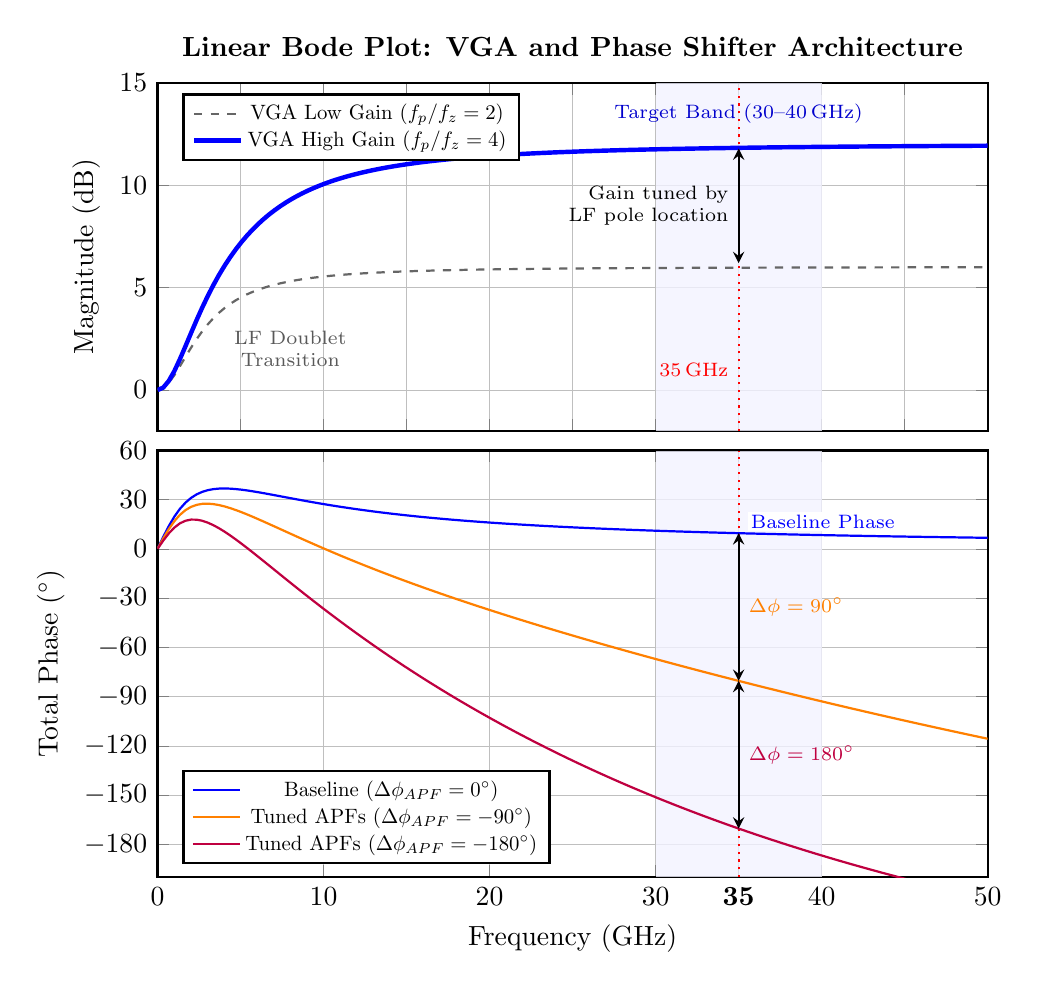
\begin{tikzpicture}

    % --- MAGNITUDE ---
    \begin{axis}[
        name=mag,
        width=\linewidth,
        height=6cm,
        xmode=normal,
        xmin=0, xmax=50,
        ymin=-2, ymax=15,
        grid=both,
        grid style={line width=.1pt, draw=gray!20},
        major grid style={line width=.2pt, draw=gray!50},
        ylabel={Magnitude (dB)},
        xticklabel=\empty,
        title={\textbf{Linear Bode Plot: VGA and Phase Shifter Architecture}},
        legend pos=north west,
        legend style={nodes={scale=0.75, transform shape}},
        thick
    ]
        \fill[blue!5, opacity=0.8]
            (axis cs:30,-2) rectangle (axis cs:40,15);
        \node[text=blue!80!black, font=\scriptsize]
            at (axis cs:35, 13.5) {Target Band (30--40\,GHz)};
        \draw[dotted, thick, red] (axis cs:35,-2) -- (axis cs:35,15);
        \node[text=red, font=\scriptsize, anchor=east]
            at (axis cs:35, 1) {35\,GHz};

        \addplot[dashed, gray!80!black, thick, domain=0.01:50, samples=150]
            {10*log10( (1 + (x/2)^2) / (1 + (x/4)^2) )};
        \addlegendentry{VGA Low Gain ($f_p/f_z = 2$)}

        \addplot[blue, ultra thick, domain=0.01:50, samples=150]
            {10*log10( (1 + (x/2)^2) / (1 + (x/8)^2) )};
        \addlegendentry{VGA High Gain ($f_p/f_z = 4$)}

        \draw[<->, >=stealth, thick] (axis cs:35, 6.2) -- (axis cs:35, 11.8)
            node[midway, left, font=\scriptsize, align=right]
            {Gain tuned by\\LF pole location};
        \node[font=\scriptsize, align=center, text=gray!70!black]
            at (axis cs:8, 2) {LF Doublet\\Transition};
    \end{axis}

    % --- PHASE ---
    \begin{axis}[
        name=phase,
        at={(mag.below south west)},
        anchor=north west,
        width=\linewidth,
        height=7cm,
        xmode=normal,
        xmin=0, xmax=50,
        ymin=-200, ymax=60,
        grid=both,
        grid style={line width=.1pt, draw=gray!20},
        major grid style={line width=.2pt, draw=gray!50},
        xlabel={Frequency (GHz)},
        ylabel={Total Phase ($^\circ$)},
        xtick={0,10,20,30,35,40,50},
        xticklabels={0,10,20,30,\textbf{35},40,50},
        ytick={60,30,0,-30,-60,-90,-120,-150,-180},
        legend pos=south west,
        legend style={nodes={scale=0.75, transform shape}},
        thick
    ]
        \fill[blue!5, opacity=0.8]
            (axis cs:30,-200) rectangle (axis cs:40,60);
        \draw[dotted, thick, red] (axis cs:35,-200) -- (axis cs:35,60);

        \addplot[blue, thick, domain=0.01:50, samples=150]
            {atan(x/2) - atan(x/8)};
        \addlegendentry{Baseline ($\Delta\phi_{APF}=0^\circ$)}

        \addplot[orange, thick, domain=0.01:50, samples=150]
            {atan(x/2) - atan(x/8) - 4*atan(x/84.5)};
        \addlegendentry{Tuned APFs ($\Delta\phi_{APF}=-90^\circ$)}

        \addplot[purple, thick, domain=0.01:50, samples=150]
            {atan(x/2) - atan(x/8) - 4*atan(x/35)};
        \addlegendentry{Tuned APFs ($\Delta\phi_{APF}=-180^\circ$)}

        \draw[<->, >=stealth, thick] (axis cs:35, 9.6) -- (axis cs:35, -80.4)
            node[midway, right, font=\scriptsize, text=orange]
            {$\Delta\phi=90^\circ$};
        \draw[<->, >=stealth, thick] (axis cs:35, -80.4) -- (axis cs:35, -170.4)
            node[midway, right, font=\scriptsize, text=purple]
            {$\Delta\phi=180^\circ$};
        \node[anchor=south west, font=\scriptsize, text=blue,
              fill=white, inner sep=1pt] at (axis cs:35.5, 10)
            {Baseline Phase};
    \end{axis}

\end{tikzpicture}
\caption{Bode plot of the VGA and all-pass phase shifter network.
         Top: gain magnitude across the \SIrange{30}{40}{\giga\hertz} band
         for two pole-zero ratios.
         Bottom: total phase at \SI{35}{\giga\hertz} is tunable over
         $180^\circ$ by adjusting the APF pole frequency.}
\label{fig:bode}
\end{figure*}

\subsection{Current-Mode Phase Interpolator}
% TODO: CML schematic and tail-current weighting
